\section{Section}
\label{section}

\subsection{Subsection}
\label{subsection}

\subsubsection{Notation, Todo and Citation}
\label{notation}
There is a stopping region \nom{$\Gamma_S$}{Stopping Layer} of width \nom[sortindex]{$\delta>0$}{Distance from boundary at which to accept a stop}.
\begin{equation}
    \alpha = \delta^2
\end{equation}
\nomenclature[z]{$\alpha$}{Distance squared}
\cite{Muller}
\todo{add a picture here}

\subsubsection{Code}
Code:
\begin{lstlisting}
void Scheduler<SchedulingAlgorithm, spacedimV>::schedule(){
// Get number of available cores
int nCores = MPI::COMM_WORLD.Get_size();

// Create instance of scheduling algorithm
SchedulingAlgorithm schedulAlgo;
// And call its scheduling method
schedulAlgo.schedule( 
        // number of available cores
        nCores,
        // List with problem weights, problem i has a computational complexity of problemSizes[i]
        problemSizes,
        // List of lists to be filled with the scheduling, problem i is calculated on all cores contained in the list problemToCore[i]
        problemToCore
);

}
\end{lstlisting}

\subsubsection{Outline}
Example of outline:
\begin{outline}
    \1 First level
        \2 Second level
            \3 Third level
        \2[+] Second level with custom symbol
    \1 Again first level
        \2[] Second level without symbol
\end{outline}
\begin{outline}[enumerate]
    \1 Numerated outline
        \2 Second level
            \3 Third level
\end{outline}

\subsubsection{Pictures}
Example of subfloats with separate labeling:
Figure~\ref{fig:strongscalingfull} shows the timing \subref{fig:sub:strongscalingfulltiming} and the efficiency plot \ref{fig:sub:strongscalingfullefficiency} for the RTE solver with the full tensor solution method.
\begin{figure}[h]
    \centering
    \subfloat[Timings]{
        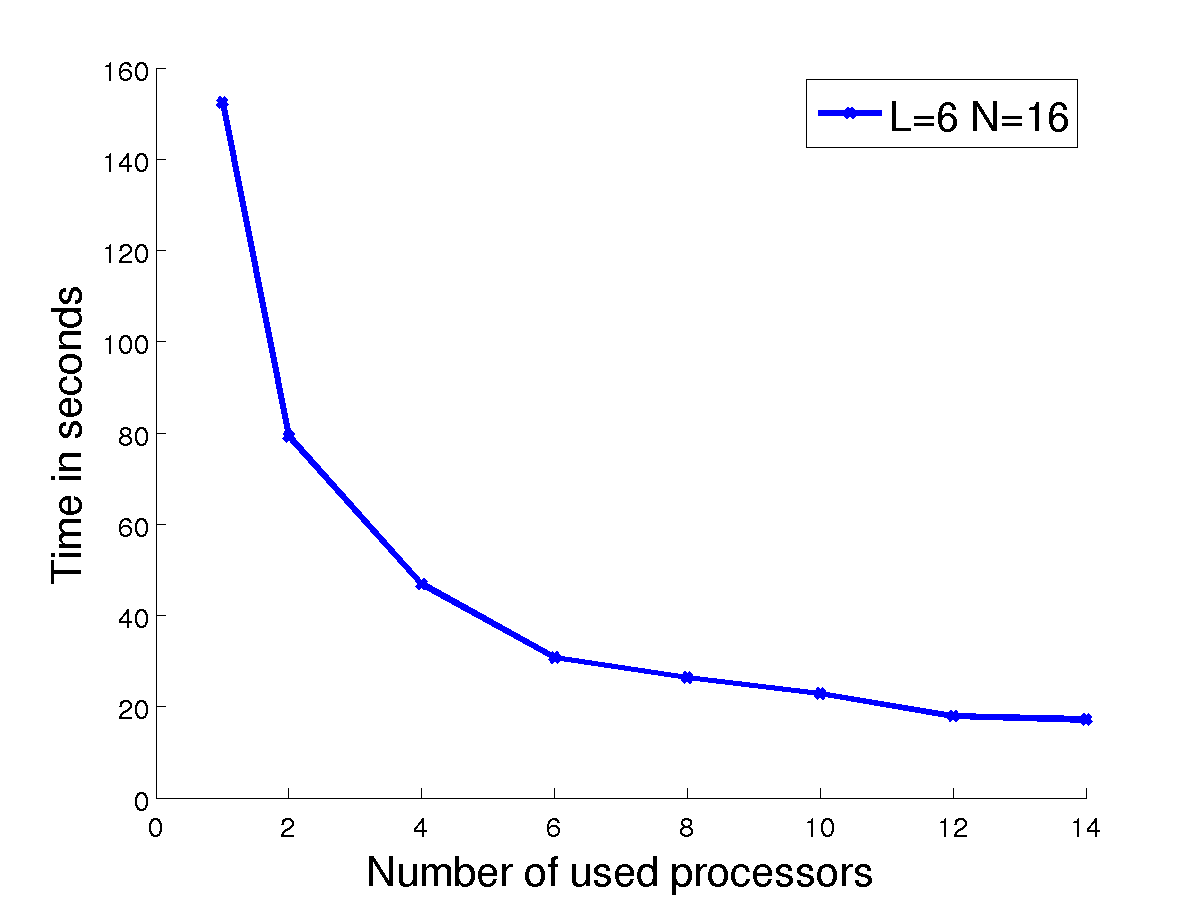
\includegraphics[height=40mm]{figures/strongscalingfulltiming.png}
        \label{fig:sub:strongscalingfulltiming}
    }
    \subfloat[Efficiency]{
        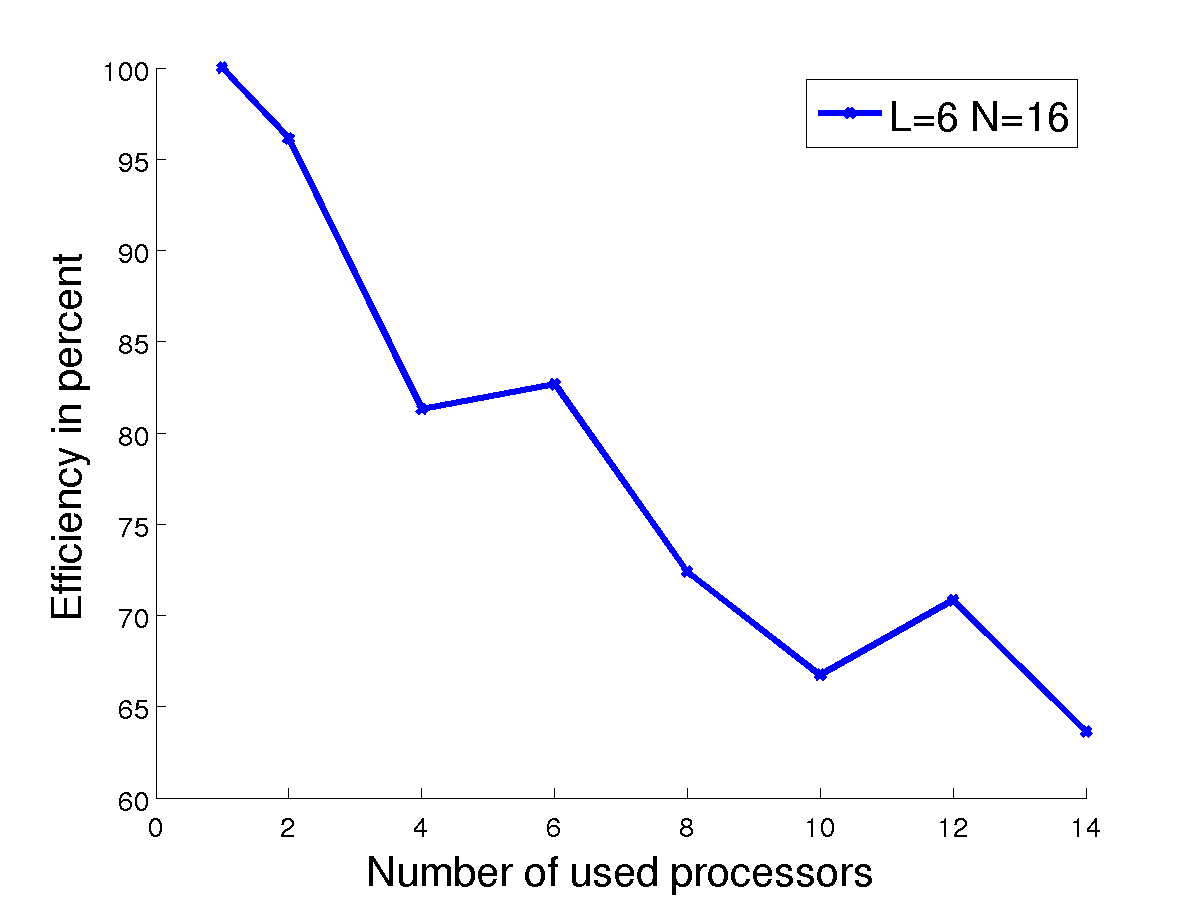
\includegraphics[height=40mm]{figures/strongscalingfullefficiency.png}
        \label{fig:sub:strongscalingfullefficiency}
    }
    \caption{Strong scaling of the RTE solver with the full tensor method. On the left the timing results are shown, on the right the according efficiency numbers are plotted.}
    \label{fig:strongscalingfull}
\end{figure}

\subsubsection{todocontent}
The todocontent environment is a customizable outline environment to help making the outline of a text.
\begin{todocontent}
    \1 This chapter should contain information about cows
    \1 And not to forget milk!
\end{todocontent}

\subsubsection{Tikz picture}
tikz is not a drawing program, but an awesome interface to one:
\begin{figure}[h]
    \centering
    \begin{tikzpicture}
        \draw[fill=lightgray] (0,0) rectangle (6,2);
        \draw[ultra thick,<->] (1,0) node[below] {x} -| (0,1) node[left] {y};
        \node[below] at (3,0) {$\u=0$};
        \node[above] at (3,2) {$\u=\Omega$};
    \end{tikzpicture}
\end{figure}
\begin{figure}[h]
    \centering
\tikzstyle{decision} = [diamond, draw, fill=blue!20, 
    text width=4.5em, text badly centered, node distance=3cm, inner sep=0pt]
\tikzstyle{block} = [rectangle, draw, fill=blue!20, 
    text width=5em, text centered, rounded corners, minimum height=4em]
\tikzstyle{line} = [draw, -latex']
\tikzstyle{cloud} = [draw, ellipse,fill=red!20, node distance=3cm,
    minimum height=2em]
    
\begin{tikzpicture}[node distance = 2cm, auto]
    % Place nodes
    \node [block] (init) {initialize model};
    \node [cloud, left of=init] (expert) {expert};
    \node [cloud, right of=init] (system) {system};
    \node [block, below of=init] (identify) {identify candidate models};
    \node [block, below of=identify] (evaluate) {evaluate candidate models};
    \node [block, left of=evaluate, node distance=3cm] (update) {update model};
    \node [decision, below of=evaluate] (decide) {is best candidate better?};
    \node [block, below of=decide, node distance=3cm] (stop) {stop};
    % Draw edges
    \path [line] (init) -- (identify);
    \path [line] (identify) -- (evaluate);
    \path [line] (evaluate) -- (decide);
    \path [line] (decide) -| node [near start] {yes} (update);
    \path [line] (update) |- (identify);
    \path [line] (decide) -- node {no}(stop);
    \path [line,dashed] (expert) -- (init);
    \path [line,dashed] (system) -- (init);
    \path [line,dashed] (system) |- (evaluate);
\end{tikzpicture}
\end{figure}
